%*----------- SLIDE -------------------------------------------------------------
\begin{frame}[t]{Introdução} 
    \transdissolve[duration=0.5]
    AUV (Autnomous Underwater Vehicle) é um veiculo subaquático autônomo, o qual não é conctado por cabos 
    a um operador e não é não tripulado.
    % COLOCAR AQUI DUAS IMAGENS DE AUVS E NA HORA FALAR SOBRE OS DIFERENTES TAMANHOS 
    % E COMO OPERAM


       %\newline
        \begin{columns}[t]
            \column{.05\linewidth}
            \column{.4\linewidth}
                \begin{itemize}
                    \item assimilar o conhecimento da interação em robots;
                    \item compreender em profundidade os conceitos de simulação, e o;
                    \item desenvolvimento da liderança em projetos \cite{Mohan2015}.
                \end{itemize}
            \column{.6\linewidth}
            \begin{center}
            %\centerline{
                \begin{figure}
                    %
\includegraphics[width=1\textwidth]{pista}
                    \caption{Pista de corrida \cite{agostini2007}}
                    \roundpic[xshift=0cm,yshift=0cm]{2.5cm}{6cm}{pista}
                    %\caption{Pista de corrida \cite{agostini2007}}
                \end{figure}
            %}
            \end{center}
        \end{columns}
%*----------- notes
    \note[item]{Notes can help you to remember important information. Turn on the notes option.}
\end{frame}
%-
%*----------- SLIDE -------------------------------------------------------------
\begin{frame}[t]{Introdução}
    \transboxout[duration=0.5]
    \framesubtitle{História}
    \begin{columns}
        \column{.1\textwidth}
        \column{.4\textwidth}
            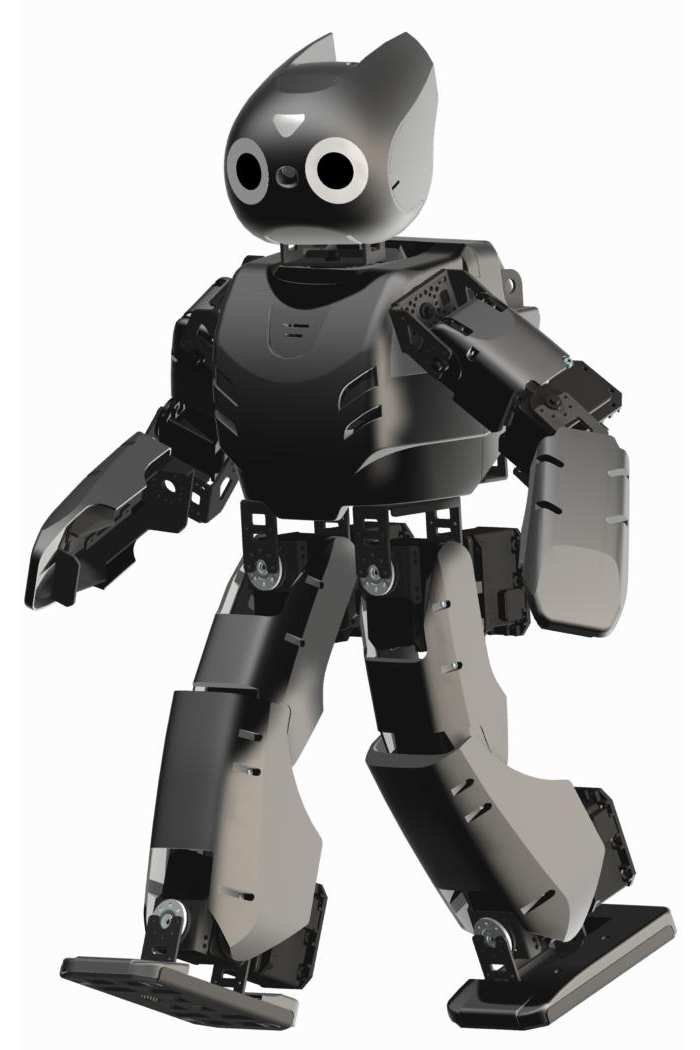
\includegraphics[width=.7\textwidth]{darwin-op}
        \column{.4\textwidth}
            \begin{itemize}
               \item Whintehead torpedo (1866)
               \item Veículo de pesquisa subaquática de propósito especial (1957)
            \end{itemize}
    \end{columns}
 %*----------- notes
    \note[item]{Notes can help you to remember important information. Turn on the notes option.}
\end{frame}
%-